%% ----------------------------------------------------------------------------------
%% GUIDELINES
%% ----------------------------------------------------------------------------------
%% - Provide details about techniques/methods that you use. Do not just write “We have
%% implemented the marching cubes algorithm”. Describe the method too, in your own
%% words. Even if it is well described in a book, you should still explain the method
%% yourself; this is part of the exercise. Also, the reader may not know the method, nor
%% can the reader be bothered to find the document that you are referring to.
%% - Discuss interesting implementation aspects, but do not include code fragments in the
%% text. Pseudo code is allowed, but mathematical formulas are preferred.
%% - Describe parameters of methods and explain which settings you used and why.
%% - Provide evidence that the method you have implemented actually works as intended.
%% - Explain how you designed a color map, a transfer function, or even your whole visualization
%% approach.

\section{MIP}\label{sec:mip}
We will start this section with explaining how the MIP raycaster was developed from the initially provided application. The initial code simply used to take a slice (plane) through the data. This plane would go through the exact center of the bounding box, and would be tilted in order to be perpendicular to the view vector \texttt{viewVec} at all times. In order to let the raycaster perform MIP, we need not only to consider the data on the slice plane, but for each pixel we need to consider all of the data on the ray from that pixel parallel to \texttt{viewVec}. We then take the maximum of these values, and project that value onto the corresponding pixel. From an implementation point of view this means that we need to introduce an additional for-loop that walks along the described ray for every pixel.

MIP is useful to make high densities stand out between other (lower) densities.
It is used for the detection of lung nodules because they stand out from pulmonary bronchi and vasculature~\cite{wikiMIP}.
MIP is a less useful method to visualize multiple layers in a 3D rendering, because only the maximal value is visible.
If the outside layer has the highest density the inside is not visible in the rendering.

\subsection{Tri-linear Interpolation}\label{subsec:tri_linear}
As explained in section \ref{sec:intro}, the value for each pixel is determined by the \texttt{getVoxel()} function using a nearest neighbor (NN) approach. In this section we will explain how this simple method is replaced by the function \texttt{getTriVoxel()}, which uses the more involved method of interpolation. In short tri-linear interpolation means that we not just copy the value of the nearest voxel, but take into account all of the eight voxels that surround the 3D-coordinate that was found along a ray. In figure \ref{fig:trilinear0}, assume the eight cube corners to be voxels with corresponding values $v_1, v_2, v_3, ..., v_8$, and point $c$ to be the coordinate on some array that has been casted through the data set. We can now determine the value of $c$ in two, practically similar ways, of which the first one is visualized in \ref{fig:trilinear0a} and the second one in \ref{fig:trilinear0b}.

\begin{figure}[h!]
    \centering
    \captionsetup{justification=centering,margin=0.5cm}
    \begin{subfigure}[t]{0.48\textwidth}
        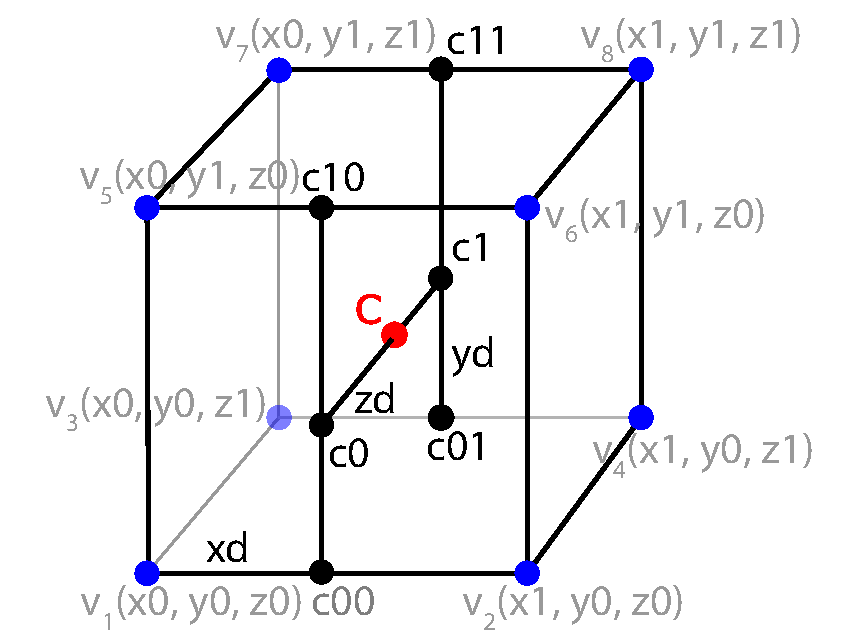
\includegraphics[width=\textwidth]{img/tri_lin_interpolation1.pdf}
        \caption{ }
        \label{fig:trilinear0a}
    \end{subfigure}
    \begin{subfigure}[t]{0.48\textwidth}
        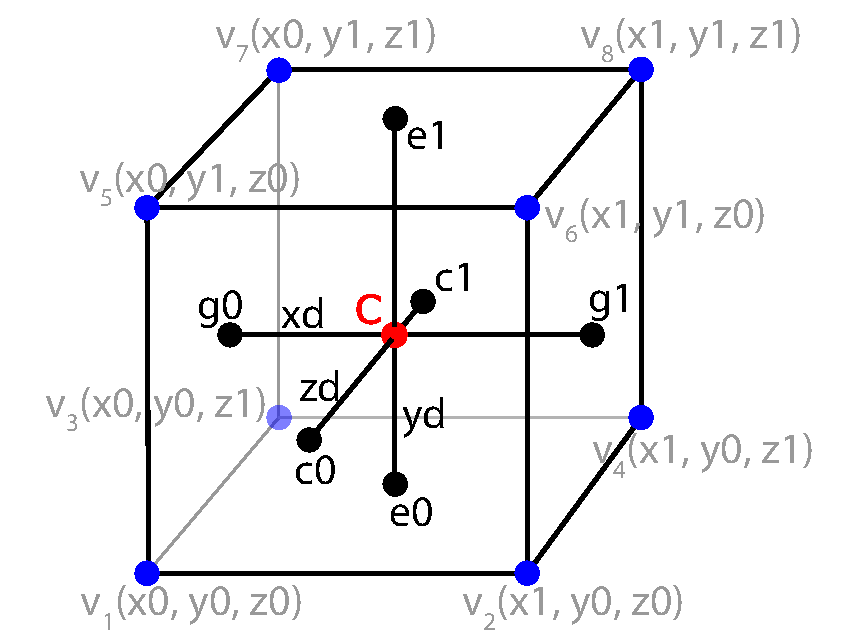
\includegraphics[width=\textwidth]{img/tri_lin_interpolation2.pdf}
        \caption{ }
        \label{fig:trilinear0b}
    \end{subfigure}
    \caption{Two different ways to obtain the Tri-Linear interpolation value of some point along a ray.}
    \label{fig:trilinear0}
\end{figure}

In both of these methods we use that:\\
$x0 = \lfloor x_c\rfloor, y0 = \lfloor y_c\rfloor, z0 = \lfloor z_c\rfloor,$\\
$x1 = \lceil x_c\rceil, y1 = \lceil y_c\rceil, z1 = \lceil z_c\rceil$

This is used to determine the values $v_1, v_2, v_3, ..., v_8$ of the eight voxels surrounding $c$. The first method \cite{wikiTriLin} (presented in \ref{fig:trilinear0a}) then interpolates the value $c$ in three steps, namely in the $x$, $y$ and $z$ direction using the following equations:

$c00 = v_1*(1-xd) + v_2*xd$\\
$c10 = v_5*(1-xd) + v_6*xd$\\
$c01 = v_3*(1-xd) + v_4*xd$\\
$c11 = v_7*(1-xd) + v_8*xd$

$c0 = c00*(1-yd) + c10*yd$\\
$c1 = c01*(1-yd) + c11*yd$

$v_c = c0*(1-zd) + c1*zd$

The second method \cite{paulBourke} calculates the value of $c$ using only one large equations. This equations interpolates the value of $c$ by the multiplying the value of each voxel with its distance to $c$, and adding all of the resulting values:

$v_c =$\\
$v_1*(1-xd)*(1-yd)*(1-zd) +$\\
$v_2*xd*(1-yd)*(1-zd) +$\\
$v_3*(1-xd)*(1-yd)*zd +$\\
$v_4*xd*(1-yd)*zd +$\\
$v_5*(1-xd)*yd*(1-zd) +$\\
$v_6*xd*yd*(1-zd) +$\\
$v_7*(1-xd)*yd*zd +$\\
$v_8*xd*yd*zd$

One of these two approaches has to be chosen, the first one seems to be the better option as it uses less calculation steps (less multiplication as well as additions). Though it does introduce some additional variables, this should not decrease the overall performance of the application.

When comparing the two different interpolation methods in \ref{fig:trilinear1}, we can see that the NN method produces a more crisp image, while the tri-linear interpolation shows a more blurry image. Though it can be argued which one of these methods may be preferred, the trilinear interpolation should in theory deliver a smoother image that may be more compelling to the eye, but shows less contrast on the other hand.

\begin{figure}[h!]
    \centering
    \captionsetup{justification=centering,margin=0.5cm}
    \begin{subfigure}[t]{0.48\textwidth}
        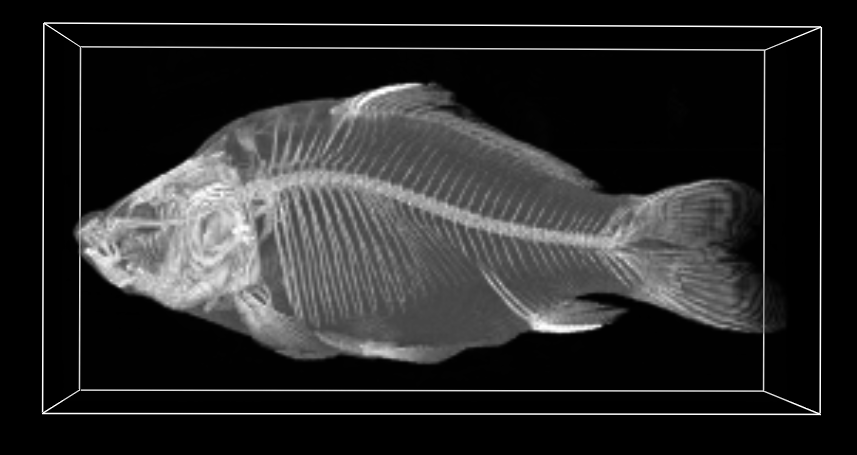
\includegraphics[width=\textwidth]{img/fish_NN.png}
        \caption{ }
    \end{subfigure}
    \begin{subfigure}[t]{0.48\textwidth}
        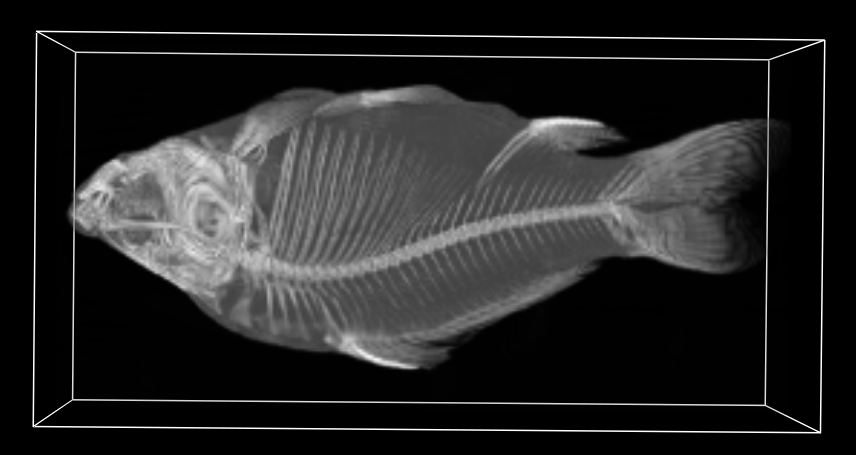
\includegraphics[width=\textwidth]{img/fish_TriLin.png}
        \caption{ }
    \end{subfigure}
    \caption{difference between NN interpolation (a) and Tri-Linear interpolation (b)}
    \label{fig:trilinear1}
\end{figure}

\subsection{Performance Enhancing}\label{subsec:perf_enh}
With the implementation of the Maximum Intensity Projection, the performance of the application decreases significantly. We therefore present several methods that improve the responsiveness of the application during user interaction.

The first one is the obvious solution of decreasing the depth resolution of the rendering. In order to this, we introduce a variable \texttt{step}, and use this variable to specify the length of the steps that are taken along each ray that is casted from the view window. When \texttt{step} is increased, the for-loop is simply walks quicker over each ray, and reaches the end of the bounding box in less calculations. In order to easily adjust the \texttt{step} value, even during runtime, an extra slider was added to the application's control panel. By moving the slider to the right, the step size increases, reducing the resolution and hence the response time of the application.
Making it possible to adjust the \texttt{step} value during runtime, also enables the user to more quickly interact with the transfer function. For every adjustment to the transfer function, the data set is rendered again, the rest of the application freezes until the rendering is completed. When this rendering takes few seconds, interaction with the transfer function becomes very cumbersome. By temporarily maximizing the \texttt{step} value (i.e. minimizing the resolution), the interaction with the transfer function can be improved drastically. Once the desired transfer function is defined, the resolution can be set back to its initial value.

Next to this, as much as possible operations within the core of the triple for-loop nest, were taken to the outer levels of this for-loop nesting. In this way, these operations are executed once, saved to some variable, and can then be used in the inner for-loops without having to recompute them. 
These variable values were the same at each inner-iteration and did not need to be recomputed each time.

For the MIP method, another obvious trick was added in order to improve performance. When walking across a certain ray, we now check every time a new highest value is found, whether this value is the maximum value. If it is, this means we can stop traversing that ray, because no higher value can ever be found (the maximum is already the highest possible value!). Obviously, this performance enhancement method does not work for the compositing rendering technique.

Another performance enhancing method that came to mind was to check in advance which part of each ray will fall inside the bounding box. In this way, the length of the most inner for-loop (walking across the ray) could be decreased. However, in order to determine whether a certain point on the ray will fall inside or outside of the bounding box, we will need to determine the coordinates of that point first. Once these coordinates are found, the function \texttt{getTriVoxel()} already checks whether this point falls within the bounding box, and hence no significant improvements could be made concerning this.

Finally, the resolution of the render is decreased automatically when the user starts rotating the render. This ensures that rotating the render can be done in a rather smooth matter, similar as proposed during interaction with the transfer function. The difference between these two is however that when rotating, the resolution is decreased automatically, instead of leaving this as a manual operation to the user.
After the mouse is released the render is computed with the original \texttt{step} resolution.
The way this automatic decrease is established is through a MouseEvent listener.
This listener saves the current mouse state and passed it to the renderer at each render update.
Whenever the mouse is pressed the \texttt{step} is overruled with a fixed resolution value, in this case 10.